\documentclass{standalone}
\usepackage[svgnames]{xcolor}
\usepackage{tikz}
\usetikzlibrary{arrows.meta}\begin{document}
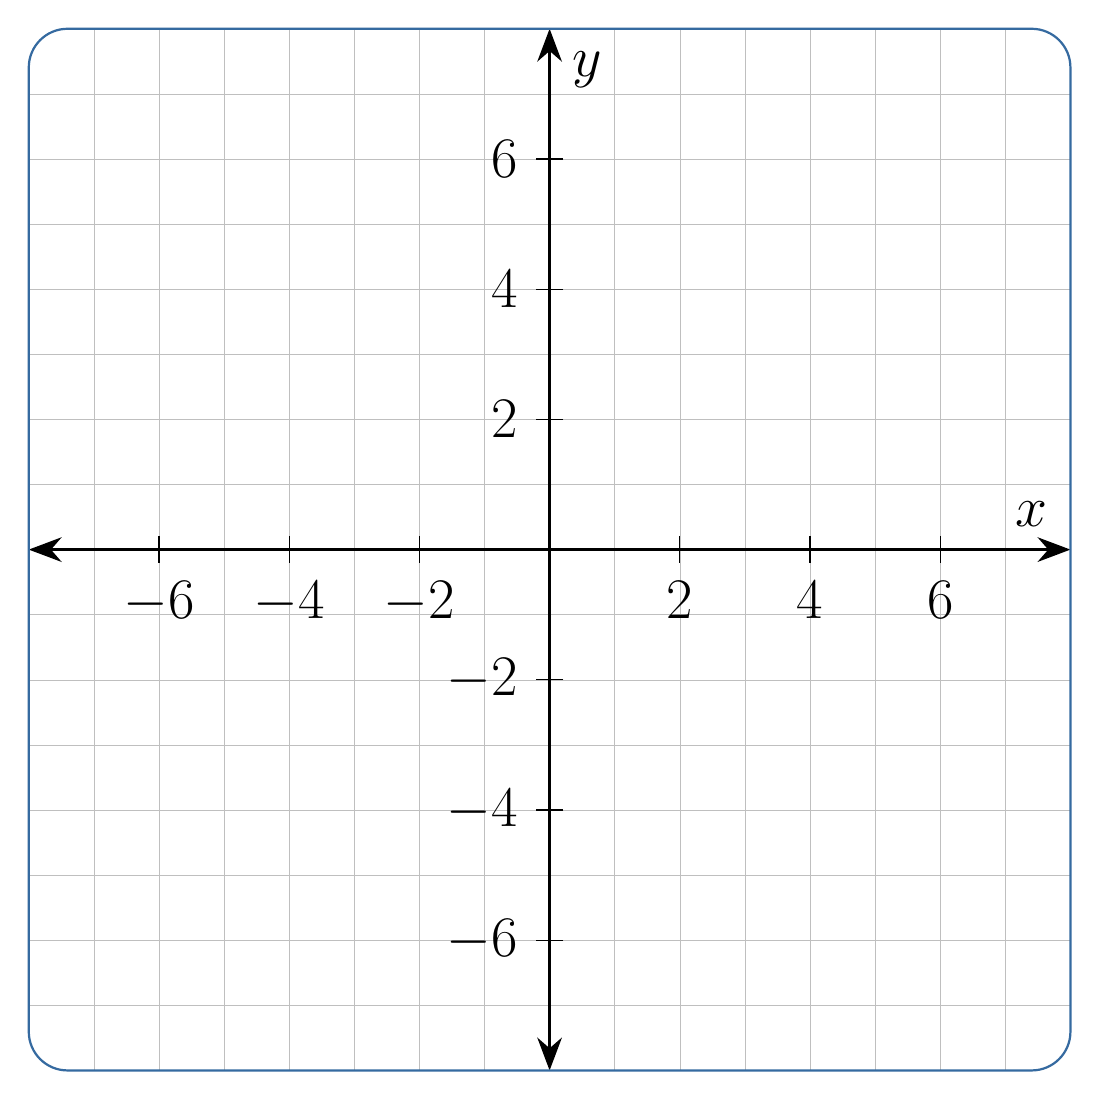
\begin{tikzpicture}[x=0.325520833333333in,y=0.325520833333333in]

\tikzset{
	>={Stealth[scale=1.8]},
	clip even odd rule/.code={\pgfseteorule},
	inverse clip/.style={ clip,insert path=[clip even odd rule]{
		(-8,-8) rectangle (8,8) }
	}
}
\definecolor{borderblue}{HTML}{356AA0}
\definecolor{fillpurple}{HTML}{A384E5}
\pgfdeclarelayer{background}
\pgfdeclarelayer{foreground}
\pgfsetlayers{background,main,foreground}
\begin{pgfonlayer}{background}
	\fill[white,rounded corners=14pt]
	(-8,-8) rectangle (8,8);
\end{pgfonlayer}
\foreach \x in {1,2,3,4,5,6,7,-1,-2,-3,-4,-5,-6,-7}{\draw[line width=0.2pt,color=lightgray] (\x,-8) -- (\x,8);}
\foreach \y in {1,2,3,4,5,6,7,-1,-2,-3,-4,-5,-6,-7}{\draw[line width=0.2pt,color=lightgray] (-8,\y) -- (8,\y);}
\huge
\draw[<->,thick] (-8,0) -- (8,0)
node[above left,outer sep=2pt]{\(x\)};
\draw[<->,thick] (0,-8) -- (0,8)
node[below right,outer sep=2pt]{\(y\)};
\foreach \x in {2,4,6,-2,-4,-6}{\draw[thin] (\x,5pt) -- (\x,-5pt) node[below]{\(\x\)};}
\foreach \y in {2,4,6,-2,-4,-6}{\draw[thin] (5pt,\y) -- (-5pt,\y) node[left]{$\y$};}
\draw[borderblue,rounded corners=14pt,thick] (-8,-8) rectangle (8,8);

\end{tikzpicture}
\end{document}
